\subsection{Taylor-Couette Flow}

\begin{figure}[!bp]
  \begin{minipage}[c]{0.6\textwidth}
      \centering
        \resizebox{0.9 \textwidth}{!}{
       \import{gfx/immersed_boundary/tcflow//}{tcsystem.pdf_tex}
      }
  \end{minipage}
  \begin{minipage}[c]{0.3\textwidth}
      \caption{Setup of the Poiseuille-flow channel.
      \label{validation:setup_tcflow}
      }
  \end{minipage}
\end{figure}

The setup of the Taylor-Couette flow is  shown in Fig. \ref{validation:setup_tcflow}.
It contains of two coaxial in z-direction oriented cylinders
with different radii $R_i$ and rotation rates $\Omega_i$. The fluid domain is given by the gap between the cylinders and
periodic in z-direction.\\
In dependency of the different domain paratemers different flow regimes can occur, criteria ...\\
We examine radial couette flow where the outter cylinder does not rotate ...\\


In constrast to the previously examined test cases this system provides different characteristics
of the flow regime at the fluid domain border. The flow along the borders is not orthogonal to the curvature of
the boundary like in the poiseuille flows we investigated before. Furthermore  new boundary
conditions are introduced, to be more precisely the Dirichlet condition is now given by $|\vec{v}(\vec{r})|_{r_i} | = |\Omega_i \times \vec{r}|$.
To begin with we want to examine the flow where the outer cyinder is not rotating, that is $\Omega_2 = 0$.

In literature this system is usually referred to as circular coutte flow (CCF) (CITE).
-description flow regimes
Furthermore we want to investigate the flow regime
below the critical instability which means that $v_z=0$. In cylindrical coordinates the problem can be reduced to a two-dimensianol coordinate system with
the coordinates $(r, \phi)$, given by the coordinate transformations $x=r\cos(\phi), y = r\sin(\phi)$.
For the non-dimensionalization we choose the default convention (CITE) $x^*=x/(R_2 - R_1)$, $v^*=v/(R_1\Omega_1)$, $t^*=tR_1\Omega_1/(R_2-R_1)$ and $\rho^*=\rho$.
The flow is then characterized by the Reynolds number $Re = \frac{\Omega R_1d}{\nu}$. With this convention the equations of motion for the steady state are given by ()
\begin{align}
    -\frac{u^2_\phi}{r} = - \frac{\partial p}{\partial r}, 0 = \frac{1}{Re}\frac{\partial}{\partial r}\left(\frac{1}{r}\frac{\partial}{\partial r}(r u_\phi)\right)
\end{align}
Integrating the equations twice leads to the solution (CITE)
\begin{align}
    u_\phi = Ar + \frac{B}{r}
\end{align}
with
\begin{align}
    A = \frac{-\Omega_1R_1^2}{R^2_2 - R^2_1} ; B = \frac{\Omega_1R^2_1 R^2_2}{R^2_2 - R^2_1}
\end{align}

\subsection{Simulations}
is below the critical instability. With this exception all other parameters where kept the same like in section ().
\clearpage
no n 512

\subsection{Results}

\subsubsection{Grid Convergence Study with comparsion to the Theoretical Solution}

The results of the grid convergence study are shown from Fig. () to Fig.().
For a better overview the results are distributed into four plots.
%The first plot shows the error of the Volumen-Penalization method,
%the second plot shows the error of the Direct-Forcing,
%the third plot shows the error of the Interpolation method and
%finally the fourth plot shows the methods with the smallest $l_2$-error
%for each method in comparsion.

In Fig. (X) the relative $l_2$-error is shown for the volume penalization method with and without the volume fraction method
for 2nd and 4th order.

For all methods an approximately linear decrease  can be observed.

The error of volume penalizations methods decrease from the order $1e-1$ to $2e-3$, with
a convergence rate of order  $\epsilon \propto N^{\approx1.16}$

The volume fraction methods results in a slighty better convergence rate of $\approx 1.65$.
The overall error is smaller, due to the faster converge rates and of order $5e-4$ for the

highest resolution. For all methods the error is in the order of $1e-2$, above a resolution of 100 points.
The best results are achieved for the 2nd order volume fraction method, except for the highest resolution.

Fig. () shows the error of the Direct Forcing method with and without the volume fraction method for 2nd
and 4th order. The error convergence is almost identical to the volume penalization method, when not using the volume
fraction method, of the order $\approx 1.2$. The convergence of the volume fraction methods is of order $\approx 1.45$
and therefore slighly weaker the for the volume penalization method.
As before the best error convergence is given by the volume fraction methond of 2nd order.

In Fig. (X) we can see the error convergence of the interpolation schemes.
Here we used 2nd and 4th order schemes, furthermore we compare the interpolation with and without the
use of the direct forcing method thus setting the velocity zero .

The 4th order interpolation with direct forcing is not shown, since the resulting velocity fields are becoming
numerically unstable. The 4th order interpolation without DF also results into a larger error but in this case
the velocity field seems to be stable the

convergence rate is of order $\approx 1.4$ and the error in the regime $1e-1$ to $4e-3$.
The best and furthermore identical results are achieved for the 2nd order interpolation with and without
use of the direct forcing method. The convergence rate is of order $\approx 2.35$ and the error
decreases from the order $2e-2$ to $1e-5$.

Finally Fig. () shows the previous methods with the best convergence rates in one plot.
In summary we can say that the overall converges rate of the interpolation method is of one order better
than the volume and direct forcing methods with volume fraction. Furthermore the relative error of the interpolation method ranges
between one and two order of magnitudes below all other methods, depending on the resolution.

\clearpage
\begin{figure}[!bp]
  \begin{minipage}[c]{0.5\textwidth}
      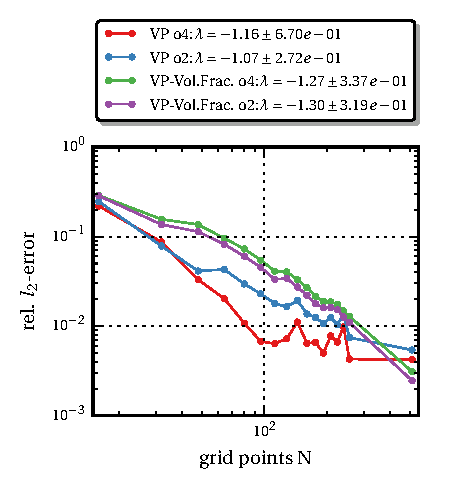
\includegraphics{gfx/immersed_boundary/tcflow/theo/vp.pdf}
      \caption{Relative $l_2$-error for different Volume-Penalization methods.}
  \end{minipage}
  \begin{minipage}[c]{0.5\textwidth}
      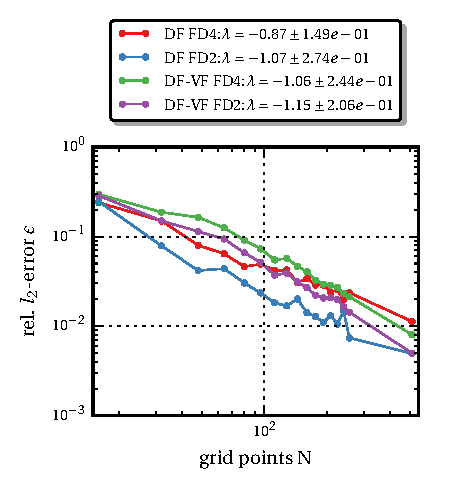
\includegraphics{gfx/immersed_boundary/tcflow/theo/df.pdf}
      \caption{Relative $l_2$-error for different Direct-Forcing methods.}
  \end{minipage}
  \begin{minipage}[c]{0.5\textwidth}
      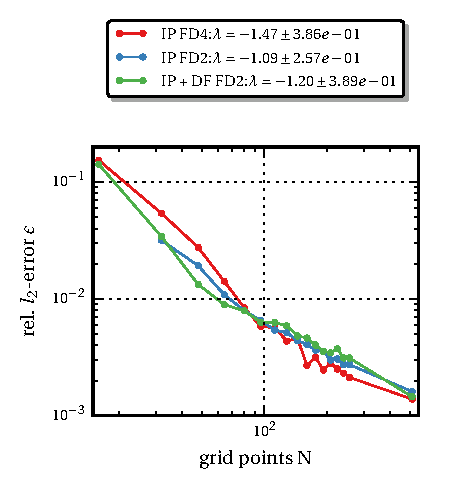
\includegraphics{gfx/immersed_boundary/tcflow/theo/ip.pdf}
      \caption{Relative $l_2$-error for different Interpolation methods.}
  \end{minipage}
  \begin{minipage}[c]{0.5\textwidth}
      \includegraphics{gfx/immersed_boundary/tcflow/theo/all.pdf}
      \caption{Relative $l_2$-error for the methods with the smallest error in comparsion.}
  \end{minipage}
\end{figure}
\clearpage

\subsubsection{Long-Term Simulations}
rho example densitiy

\subsubsection{Velocity Profiles}

\subsection{Discussion}
